\chapter{Présentation de l'entreprise}
\label{PresentationEntreprise}

MobiGIS\footnote{site de l’entreprise \url{http://www.mobigis.fr/}} se présente comme une entreprise au coeur de l’innovation, dont l’activité est d’apporter des réponses sur-mesure aux besoins de ses clients en matière de \textbf{géomatique}, notamment lorsqu’elle est appliquée aux enjeux de transport et de mobilité. MobiGIS est une société innovante éditrice de solutions dans le domaine des Systèmes d’Information Géographique (SIG). 
Elle intervient dans les thématiques : de l’environnement et du développement durable ; de la mobilité des personnes ; du transport et de la logistique (cf. Figure \ref{fig1}).\\

Ses équipes font de la conception, mise en \oe uvre et déploiement d'architectures SIG, développement d’applications de cartographie web et mobiles, études de transports, solutions de prévention des risques, etc. L’entreprise est compétente dans l’édition de logiciels SIG, le conseil et les services en SIG, la R\&D liée aux NTIC.\\

\section{Une activité centrée sur les services SIG et l'édition de logiciels}

Les clients de MobiGIS sont des industries, la grande distribution, les collectivités locales, et les intégrateurs et société de services en ingénierie informatique (SSII) (cf. Figure \ref{fig2}). L’entreprise développe en particulier une activité d’édition de logiciels. Ceux-ci permettent de faire des analyses multiples : territoire, pollutions, démographie, etc., d’élaborer des plans de déplacement urbain et entreprise, d’étudier et de préparer la réorganisation des réseaux multimodaux et la création de nouvelles infrastructures de transport. Elle compte parmi ses clients des Autorités Organisatrices de Transports (ex:Tisseo), des bureaux d’études, des sociétés de consulting immobilier et des agences d’urbanisme.\\

\begin{figure}[t]\label{fig1}
\centering
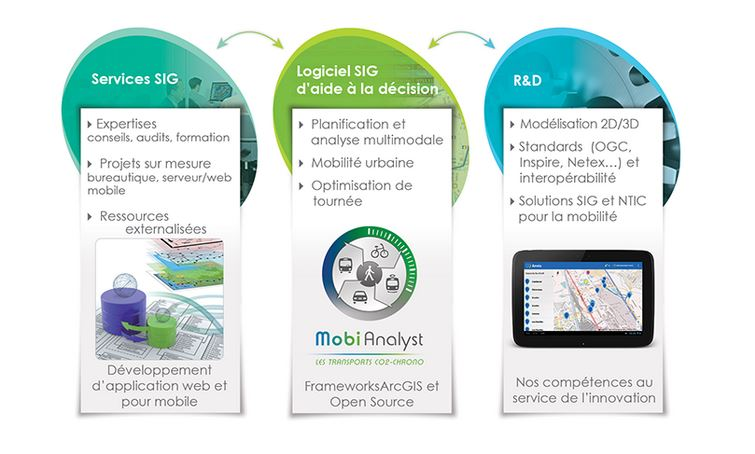
\includegraphics[width=12cm]{images/fig1_solutionsMobigis.JPG}
\caption{Offres de services Mobigis}
\end{figure} 

\begin{figure}[t]\label{fig2}
\centering
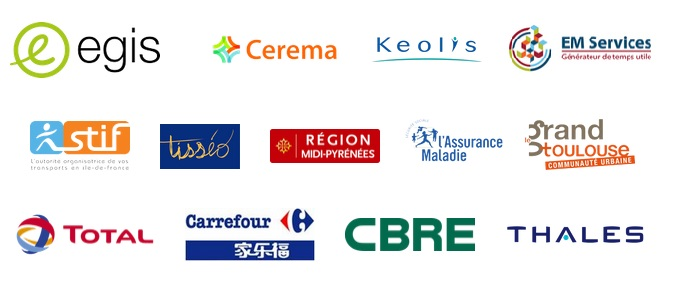
\includegraphics[width=12cm]{images/fig2_referencesMobigis.JPG}
\caption{Exemples de clients Mobigis}
\end{figure} 

\section{Mettre en avant la R\&D pour renforcer l'innovation}

MobiGIS consolide son expertise en donnant une place importante à la R\&D (Recherche et Développement). Plusieurs exemples peuvent être mis en avant. 
Le projet AMORES, collaboration labellisée par l’Agence Nationale de la Recherche, s’intéresse à la sécurisation des données géolocalisées et à la protection de la vie privée dans les services de mobilité. Au sein de ce projet, MobiGIS s’est focalisé sur le covoiturage dynamique, le calcul en temps réel des itinéraires de transport multimodal et les réseaux sociaux mobiles.\\ 
Des applications web SIG 2D/3D de repérage en gare a également été réalisée pour les Pays de la Loire. Ces applications cartographiques interactives fournissent aux personnes à mobilité réduite (PMR) des informations spécifiques à leurs handicaps présentant les services accessibles et disponibles en gare et les cheminements pour y parvenir. \\
Enfin, MobiGIS donne l’exemple d’un prototype développé pour la RATP. Celui-ci permet des comparaisons d’itinéraires voyageurs et des analyses des cheminements dans les stations RER à Paris. Ce projet comprend une intégration de données : plan bâti 2D/3D, voirie, voies ferrées, bus, etc., le calcul des cheminements dans la station sur différents niveaux (pris en compte des escaliers et équipements) et enfin l’analyse des flux voyageurs et temps de parcours selon les profils piétons. 

\section{Historique de l'entreprise}
\renewcommand{\labelitemi}{\textbullet}
\begin{itemize}
\item 2007 
    - Création de la société MobiGIS par Frédéric SCHETTINI 
		
    - Le projet de création de société a obtenu le titre de « projet de création d’entreprises innovantes » par le pôle innovation de la Chambre de Commerce et d’Industrie de Toulouse 
		
    - La société MobiGIS est accompagnée par Oséo Midi-Pyrénées 
    
		- MobiGIS obtient le statut de Jeune Entreprise Innovante (JEI) 
\\
\item 2008 
    - Pise en place d’une démarche active de développement des activités de MobiGIS en Chine 
    
		- Obtention du Prix TOTAL de l’Innovation IT 
    
		- Phase intensive de Recherche Développement 
    
		- Début de collaboration avec le CNRS/LAAS 
    
		- Labellisation du projet POTIMART par la PREDIM 
\\
\item 2009 
    - Emménagement sur le site de Grenade-sur-Garonne (31) 
    
		- MobiGIS intègre le groupement CECILE, composé de PME Toulousaines spécialisées dans la géolocalisation 
    
		- MobiGIS rejoint l’association JEInnov 
\\
\item 2010 
    - MobiGIS accompagne le ministre des transports en Chine 
    
		- Labellisation par la Plateforme de Recherche et d’Expérimentation pour le Développement de l’Information Multimodale (PREDIM) du projet CAMERA 
    
		- MobiGIS recrute un Volontaire International en Entreprise (VIE) pour intensifier son développement en Chine 
    
		- Soutien de la Région de Midi-Pyrénées pour un Contrat d’appui 
\\
\item 2011 
    - Commercialisation du progiciel MobiAnalyst 
    
		- Soutien de la CCIT et d’HGI Tech pour intensifier son développement commercial 
    
		- Recrutement d’un chef de projets SI et d’un ingénieur commercial 
\\
\item 2012 
    - L’équipe MobiGIS s’étoffe et compte désormais plus de 10 collaborateurs 
    
		- Prix de l’innovation au Toulouse Space Show et lauréat du concours Open Data « Défi numérique Toulouse Métropole » 
    
		- Ouverture d’un bureau à Paris 
    
		- Adhésion à l’Aerospace Valley 
    
		- Participation à 10 congrès dont l’ITS World à Vienne 
\\
\item 2013 
    - Signature de nouveaux contrats avec le groupe Total, Carrefour China, et l’APEM 
    
		- Lancement de la solution Anvio et de la V2.3 de MobiAnalyst 
\\
\item 2014
    - MobiAnalyst© remporte le prix de meilleure application de l'année !
    
		- Ouverture d'un bureau au Canada pour intensifier l'activité en Amérique du Nord
    
		- Premier Workshop MobiGIS organisé en septembre 2014 

\end{itemize}



\section{Ressources de l'entreprise}

Les logiciels et les compétences humaines à l’\oe uvre à MobiGIS sont au c\oe ur de l’activité, et même de la réputation de l’entreprise. Les ressources matérielles et immatérielles sont étroitement liées dans ce contexte. Ainsi, les logiciels ont besoin de l’équipe pour être maintenus, valorisés et améliorés, et l’équipe a besoin de ressources technologiques pour mener à bien les projets de l’entreprise et de ses partenaires.\\ 

Les compétences humaines permettent à l’entreprise de mener à bien des projets SIG de design et implémentation d’architecture logicielle, de systèmes de gestion de bases de données spatiales et enfin de développements bureautique, serveur, web et mobile. \\

L’entreprise héberge également les compétences nécessaires pour mener à bien des missions de conseil, d’audit et de consulting. Elle peut établir des états des lieux, des analyses et des préconisations. Enfin, MobiGIS propose des formations sur ses progiciels sur site ou à distance (web seminars / webinars). En septembre 2014, l’entreprise a également organisé un séminaire gratuit et délocalisé en IDF. Cet événement, qui a attiré des professionnels du secteur des transports est une manière de présenter les produits et compétences de l’entreprise, de nouer des contacts et de convaincre des clients potentiels. Ce genre d’événement, ouvert à tous est également propice à des rencontres avec des concurrents susceptibles de devenir de nouveaux partenaires.\\

Ces ressources peuvent être externalisées auprès des clients qui le souhaitent, de manière à mettre à leur disposition des chefs de projets, des experts SIG (anciens d’ESRI, informaticiens spécialisés), des géomaticiens au profil plus généraliste et des développeurs IT. De fait, les employés se déplacent régulièrement chez les clients de l’entreprise et développent avec eux une relation dans la durée, le temps de monter les projets, de créer et d’installer les solutions, d’apporter des retouches si nécessaire et de former les clients à l’utilisation des produits. \\

Les technologies maîtrisées par MobiGIS sont les SIG propriétaire, les SIG libres, les langages de programmation logicielle, web et mobile. Les SIG propriétaire est en premier lieu ArcGIS, mais MapInfo, GeoConcept et Google Maps sont également cités. Actuellement, l’entreprise s’inscrit dans la tendance, dans le sillage d’ESRI, de ne plus seulement proposer des solutions desktop (qui imposent d’installer ArcGIS Desktop, etc.) et de proposer davantage de solutions à distance, plus souples (et moins onéreuses pour l’acheteur), notamment sur le modèle (et en utilisant le support) d’ArcGIS Online. Les SIG libres présentés sont QGIS, GeoServeur, PostGIS, OpenLayers, mais ils n’ont pas été abordés au cours du stage. \\

Les langages maîtrisés par les informaticiens et géomaticiens de l’entreprise sont notamment Java, C++, C#, Python… ils permettent de programmer les progiciels de l’entreprise. Les développeurs font un effort de « propreté » dans leurs scripts afin de faciliter les révisions à venir. Cela est d’autant plus nécessaire dont les évolutions sont fréquentes, afin de continuer à être compatible avec les autres logiciels et sur les systèmes d’exploitation du marché qui évoluent rapidement. Enfin, cet effort doit permettre de faciliter une bonne prise en main des codes par les développeurs, dans un contexte où le turnover et la répartition fragmentaire des tâches fait que de nombreuses personnes sont susceptibles de travailler sur différentes parties d’un code, au risque d’en perdre la vision d’ensemble. Enfin, l’équipe MobiGIS pratique couramment les langages du web : HTML 5, JavaScript, PHP, CSS et des supports mobiles : IOS, Android, qui prennent une importance croissante en raison de l’évolution des pratiques de la mobilité et du besoin accru de flexibilité. \\

Parmi les missions effectuées au cours du stage, il y en a eu une directement liée à ce contexte de développement d’applications. Il s’agissait de tests effectués sur le module Datawizard (Python / SQL), qui permet la création de réseaux MobiAnalyst.\\
